\chapter{Learning to learn}
\label{chap:learn}

Learning to learn or meta-learning is growing increasingly popular in machine learning and robotics. It can refer to learning hyper-parameters for learning methods to overcome the need for hand-tuning these, from simulation to hardware or across tasks. In our case, we use simulations to extract information that will enhance the rate of learning on hardware. 

In this chapter we describe two ways of adding data from simulation to hardware optimization. We start by learning feature transforms in simulation and then use them to speed up learning on hardware. The second approach is to learn a robust policy directly in simulation and implementing it on hardware. The two approaches have different advantages. While learning features lets us use very inaccurate simulations, and still learn efficiently on hardware, it needs expert input in designing the controller structure. On the other hand, directly learned policies can have very small amount of expert input and still successfully learn walking controllers. However, we show that adding structure in the form of expert knowledge can greatly help in the rate of transfer of learned policies between simulation and hardware.

We start by describing a hand-designed locomotion-specific feature transform which is inspired from the Determinants of Gait walking metric \citep{inman1953major}. Next, we explain an automatic way of learning a feature transform from data using neural networks. Both these approaches aim at collecting data by running a lot of simulations (``Big simulation") and use it to extract behavioral information about the controller space. This information will later be used for hardware and perturbed-simulation experiments that demonstrate sample-efficiency at learning controllers.

\section{Distance metrics from simulation}
In this section, we describe our proposed bipedal locomotion specific feature transform, followed by a more general transform learned from data. Once these feature transforms are collected for a range of controllers in simulation, they are then used in the optimization of controllers on hardware. The general pipeline of this approach is shown in Figure \ref{fig:approach}.

\begin{figure}
    \centering
    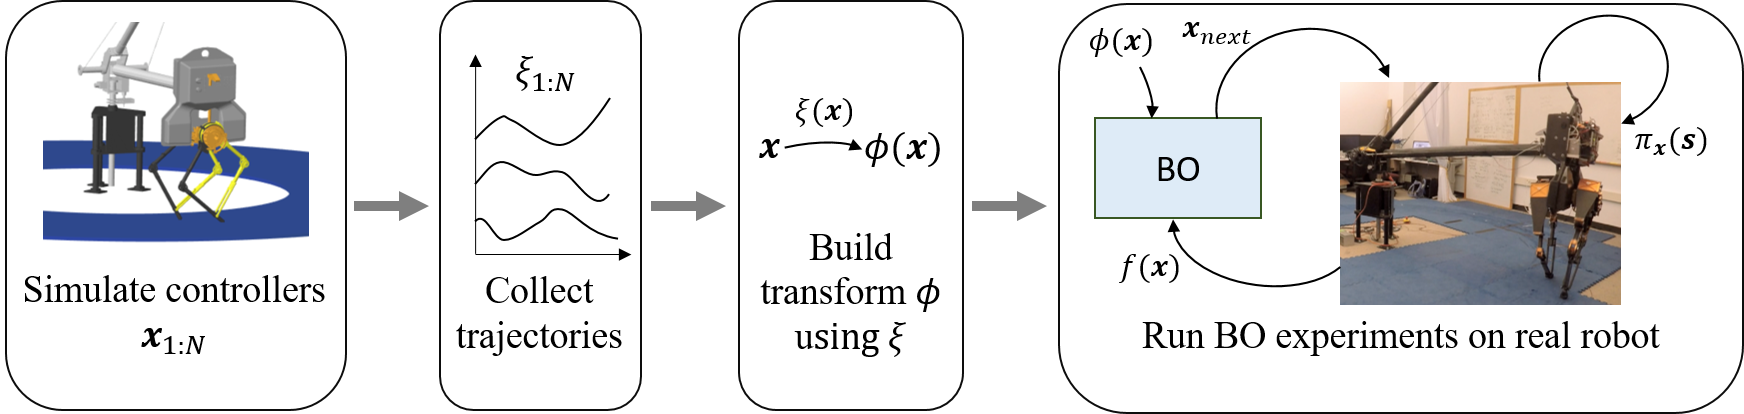
\includegraphics[width=0.9\textwidth]{img/approach.png}
    \caption{Overview of our proposed approach. Here, $\pi_{\pmb{x}}(\pmb{s})$ is the policy (described in Section~\ref{sec:dp});  $\pmb{x}$ is a vector of controller parameters; $\pmb{s}$ is the state of the robot; $\xi(\pmb{x})$ is a trajectory observed in simulation for $\pmb{x}$; $\phi(\cdot)$ is the transform built using $\xi(\pmb{x})$. $f(\pmb{x})$ is the cost of $\pmb{x}$ evaluated on hardware. BO uses $\phi(\pmb{x})$ and evaluated costs $f(\pmb{x})$ to propose next promising controller $x_{next}$. }
    \label{fig:approach}
\end{figure}

\subsection{Constructing Flexible Kernels using Simulation-based Transforms}

High dimensional problems with discontinuous cost functions are very common with legged robots, where slight changes to some parameters can make the robot unstable. This can adversely affect the performance of Bayesian optimization, as it depends on interpolation to decide the next point to sample. However, an informed feature transform can transform the space into a more continuous, easy to approximate and optimize landscape. \cite{wilson2014using} show that using trajectory information in the kernel can speed up learning for classic reinforcement learning problems such as mountain car, over a squared-exponential kernel. We leverage trajectories from simulation to build such a feature transform for legged robots.

Feature transforms $\phi(\pmb{x})$ from simulation for a given controller $\pmb{x}$ can be used to create an informed kernel $k_{\phi}(\pmb{x}_i, \pmb{x}_j)$ for BO on hardware:

\begin{align}
    \pmb{t}_{ij} \!=\! \phi(\pmb{x}_i) \!-\! \phi(\pmb{x}_j) \\
    k_{\phi}(\pmb{x}_i, \pmb{x}_j) = \sigma_k^2 \exp\Big(- \tfrac{1}{2} \pmb{t}_{ij}^T  \diag(\pmb{\ell})^{\!-\!2} \pmb{t}_{ij} \Big)
\end{align}
Note that the functional form above is same as that of Squared Exponential kernel, if considered from the point of view of the transformed space, with $\phi(\pmb{x})$ as input. While this kernel is stationary as a function of $\phi$, it is non-stationary in $\pmb{x}$. $\phi$ can bring closer related parts of the space that would be otherwise far apart in the original space. BO can then operate in the space of $k_{\phi}$, which is `informed' by simulation.

\subsection{A bipedal locomotion specific transform}

The proposed locomotion feature transform is a generalization of the Determinants of Gaits (DoG) used by physiotherapists to evaluate the quality of human walking \citep{inman1953major}. We modify these features to look at the following aspects of bipedal walking:

\begin{enumerate}
    \item {\bf{$M_1$ : Swing leg retraction}} -- We look at the swing leg trajectory in swing and if the maximum leg retraction is more than a threshold, we set $M_1 = 1$. Otherwise, $M_1 = 0$. Higher swing leg retraction is better for disturbance rejection in the presence of obstacles, etc. Hence, a controller is less likely to fall if $M_1 = 1$.
    
    \item {\bf{$M_2$ : Center of Mass height}} -- We look at the Center of Mass (CoM) height at the start and end of each step. If the CoM height stays about the same (change is below a threshold), we set $M_2 = 1$. Otherwise, $M_2 = 0$. This metric checks that the robot is not falling across steps, but allows changes in CoM height within a step. Human-like walking typically exhibits a oscillatory CoM movement within a step, while with a linear inverted pendulum controller, the CoM height stays constant through the step. Thus, looking at just the CoM height at the start and end of a step includes both these situations and makes sure that the controller isn't falling. Thus, $M_2 = 1$ controllers are likely to walk.
    
    \item {\bf{$M_3$ : Trunk lean}} -- We compare the mean trunk lean at the start and end of a step, and if the average lean is about the same (change is below a threshold), we set $M_3 = 1$. Otherwise, $M_3 = 0$. This ensures that the trunk is not changing orientation between steps, but allows the lean to change within a step. Again human-like walking typically exhibits a oscillatory torso movement within a step, while typical walking controllers maintain a constant torso lean. Thus, looking at just the torso lean at the start and end of a step includes both these situations and makes sure that the controller isn't falling. Thus, $M_3 = 1$ controllers are likely to walk.
    
    
    \item {\bf{$M_4$ : Average walking speed}} -- We evaluate the average speed of a controller per step and set $M_4 = v_{avg}$. Unlike the other metrics, $M_4$ is not binary and helps distinguish between controllers that satisfy all conditions of $M_{1-3}$. In general, faster walking controllers could be better, though that depends on the desired walking speed. $M_4$ helps distinguish controllers that score the same of $M_{1-3}$ but lead to different behaviors in simulation.
    
\end{enumerate}

The step metrics $M_{1-4}$ are collected per step $i$ and summed over the total number of steps $N$. 
\begin{align}
\label{eq:dog}
 score^i = \sum_{j=1}^4 M^i_j  \\
 score_{DoG} = \sum_i^{N} score^i
\end{align}

In general, a higher score implies better performance of a controller for $M_{1-3}$. If $M_{1-3}$ are 0 for a particular controller, it is likely to fall. On the other hand if $M_{1-3}$ are 1 for a controller, it is likely to walk. However, the score doesn't have a fixed relationship to a particular cost function. The cost depends on the specific desired behavior/outcome.

Controllers that chatter (step very fast, with step time less than $100ms$) can have a large number of steps before falling. Since this could lead to a misleadingly high score, the DoG score is scaled by the fraction of time the simulation walked before falling. If the simulation terminated at time $t_{sim}$ and the desired time for simulation was $t_{max}$, the final DoG score $\phi$ becomes:
\begin{equation}
    \phi = score_{DoG} \cdot \frac{t_{sim}}{t_{max}}
\end{equation}

$\phi$ defines a reparameterization of a controller from the original space of controller parameters into a 1-dimensional space. We use $\phi$ to define a 1-dimensional kernel that uses the Determinants of Gait scores. The functional form of this kernel is the same as Squared Exponential kernel. However, instead of Euclidean distances of points in the original space, we use distances between the DoG scores of the points:
\begin{align}
    k(\pmb{x}_i, \pmb{x}_j) \rightarrow k(\phi(\pmb{x}_i), \phi(\pmb{x}_j)) \\
    k_{DoG}(\pmb{x}_i, \pmb{x}_j) = \sigma_k^2 \exp\Big(- \frac{1}{2 \pmb{l}^2} \|\phi(\pmb{x}_i) - \phi(\pmb{x}_j)\|^2 \Big),
\end{align}
where hyperparameters $\sigma_k^2, \ \pmb{l}^2$ are signal variance and length scale respectively. We refer to $k_{DoG}$ as `\dogkernel' in the following sections.
To speed up calculation of kernel distances during optimization, we pre-calculate $\phi$ for a large grid of points in simulation. We run short simulations of each point/controller, evaluate $\phi$ and store it in a large look-up table.

\begin{figure}
    \centering
    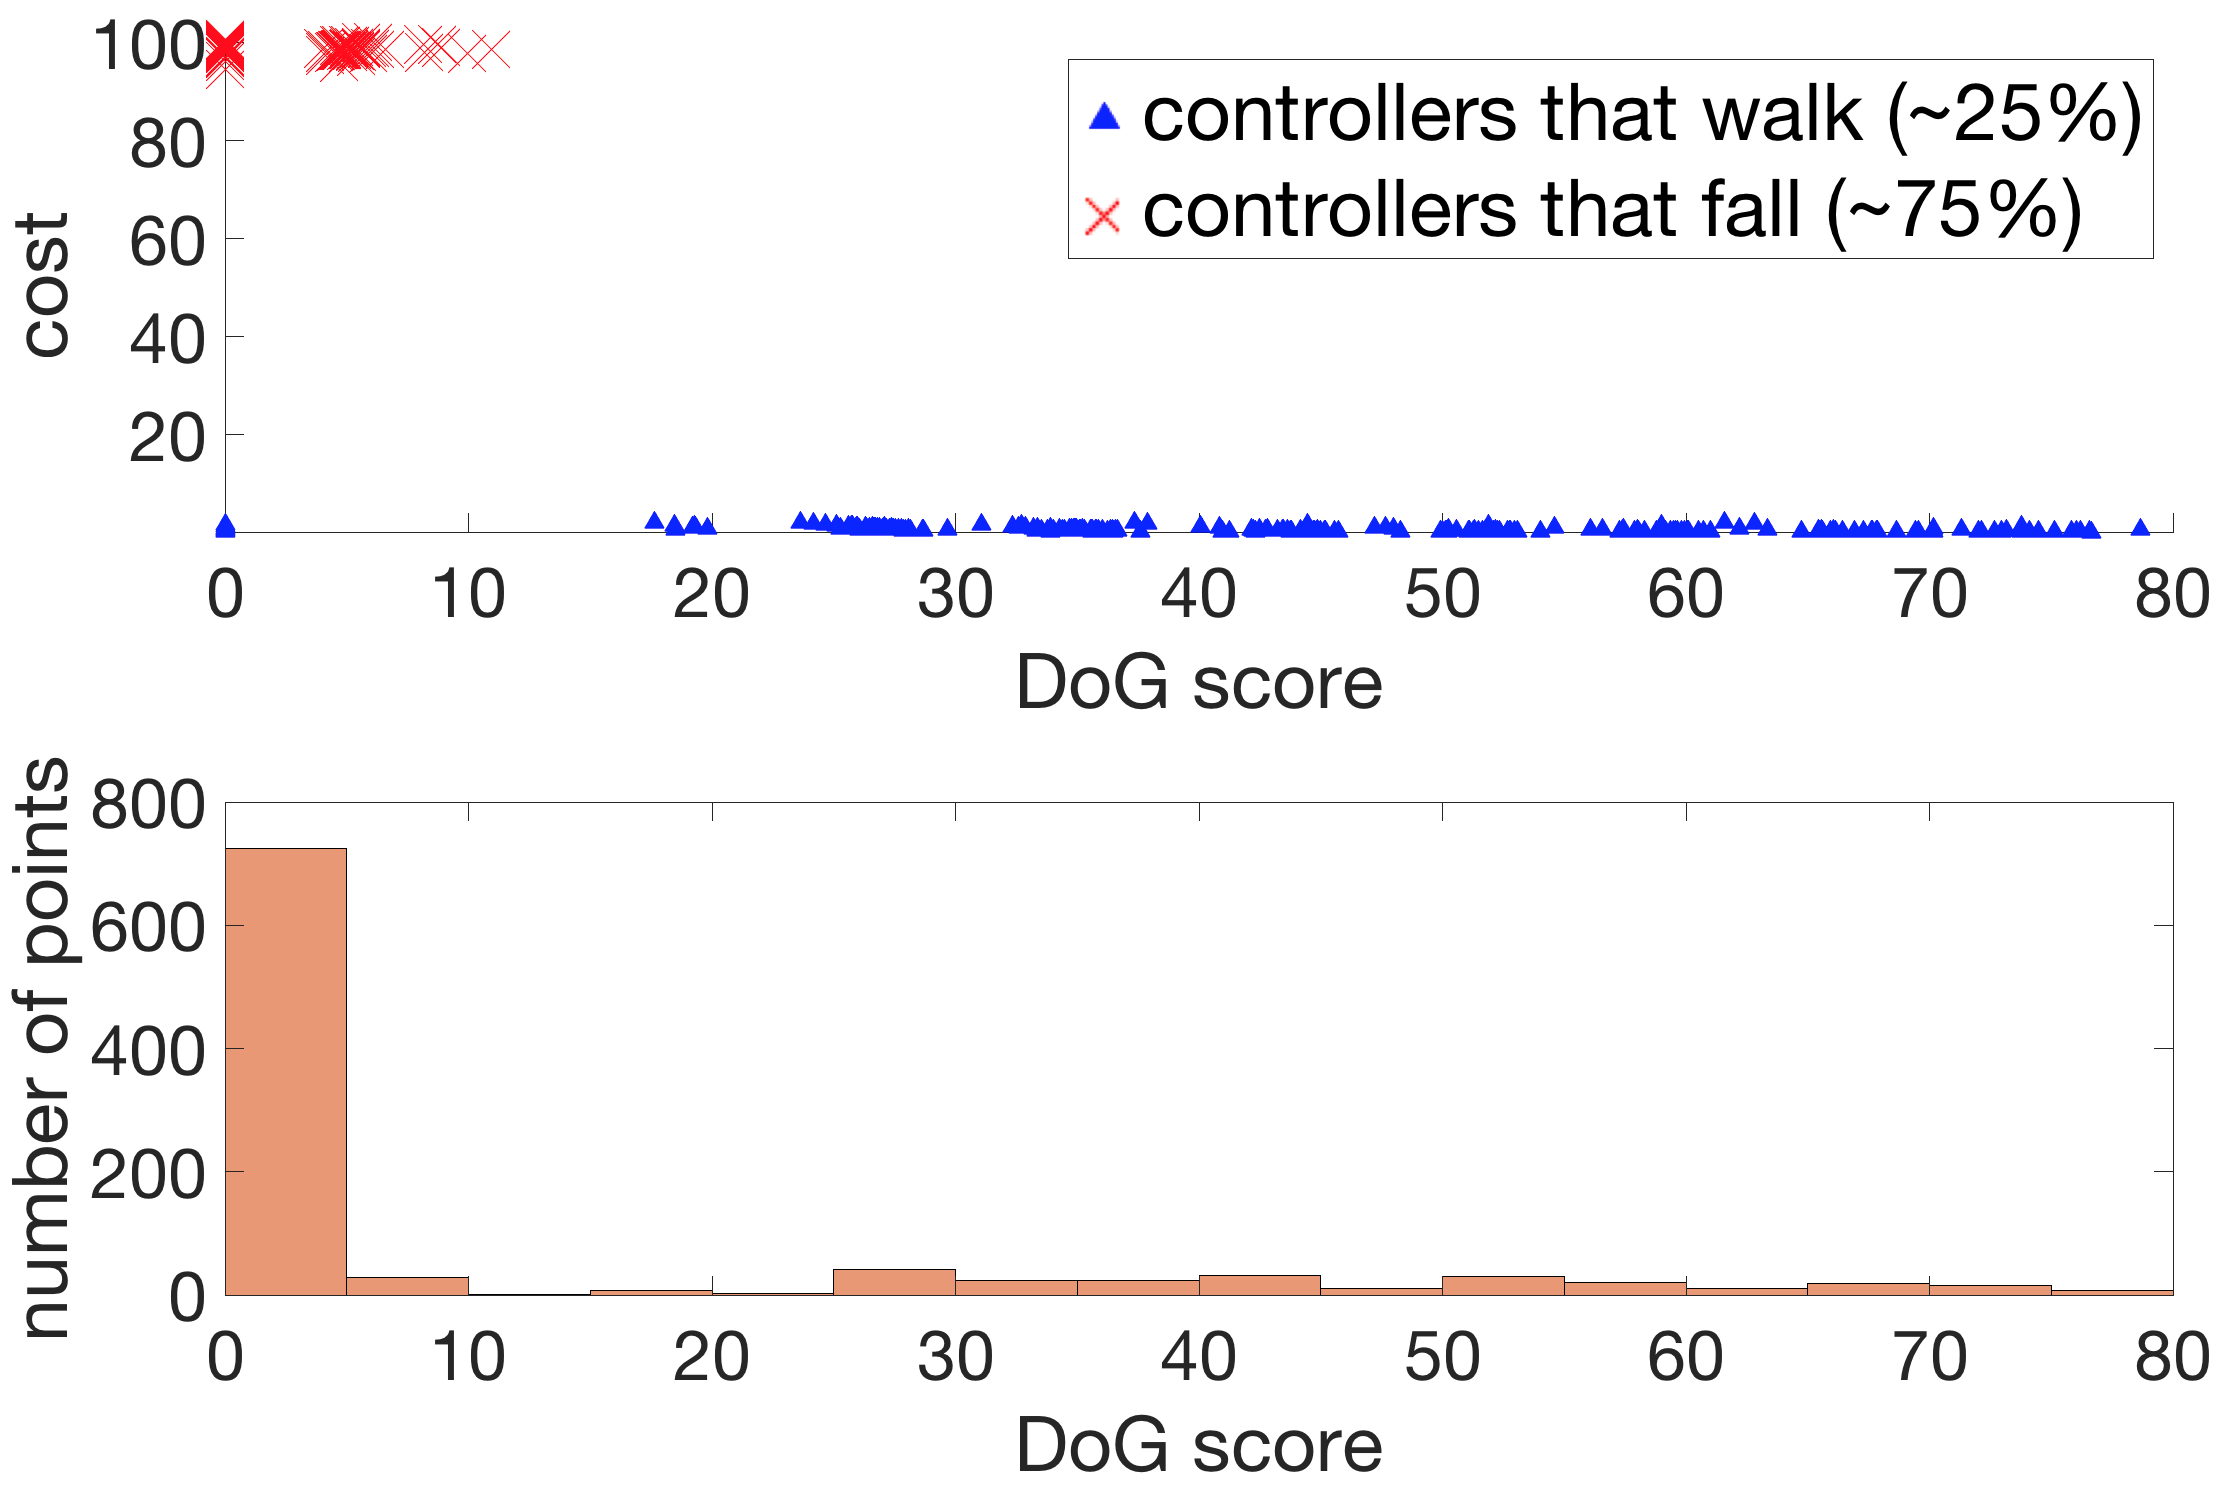
\includegraphics[width=0.75\textwidth]{img/dog_vs_cost_and_hist.png}
    \caption{\small{DoG score vs cost for 1000 randomly selected controller parameters (controller and cost from Sections~\ref{sec:raibert_cont},\ref{sec:exps_sim}). Lower DoG scores usually lead to higher costs and falling. A few points that step very fast (chatter)  don't fall in simulation, so can have low cost and low DoG score. But such points are very likely to fall on hardware.}}
            \vspace{-5mm}
    \label{fig:dogvsfit}
\end{figure}

The DoG score helps cluster controllers based on their behaviour in simulation. The hope is that behavioral cues like the ones described in metrics $M_{1-4}$ have a higher chance of transferring between simulation and hardware  than costs. On hardware, once we have evaluated a controller with a particular value of $\phi$, we expect controllers with similar values of $\phi$ to have a similar cost. This roughly splits the cost function landscape, separating points that can potentially walk, and those that cannot, as shown in Figure \ref{fig:dogvsfit}. Suppose we sample an unstable point with a low $\phi$ score and obtain a high cost on hardware (we can also seed our search with such points). We can then be fairly certain of other unstable points from simulation doing poorly as well. As a result, we can focus on potentially promising points to sample -- making the search more sample efficient and biased towards sampling safe points.


Note that in Equation \ref{eq:dog}, metrics $M_{1-4}$ are weighed equally when summing up. This simple, low-dimensional version of a feature transform is very efficient at finding walking controllers as it groups all non-walking controllers as one and separates them from all walking controllers. However, it is not good for distinguishing between walking controllers. In other words, if we are only searching for reasonably good walking controllers, and do not care about optimizing the quality of walking of each controllers, the 1 dimensional kernel is ideal for quickly reaching such a controller. However, if we care about the quality of walking, for example, we would like to walk at a particular speed, or minimize metabolic energy, the 1 dimensional kernel isn't ideal for distinguishing between such controllers.
A small but useful addition could be to learn the weights for a 4-dimensional feature transform $[M_1, M_2, M_3, M_4]$ using Automatic Relevance Determination (ARD), described in \cite{GPsMLBook}, before summing up. This would enable us to weigh the 4 metrics depending on their importance for a particular task, controller or robot. Another addition would be to use a 4-dimensional kernel, which might be less sample-efficient, but more robust to mismatch between simulation and hardware, as well as help optimize particular cost functions better. 


\subsection{A feature transform from learned data}

While hand-designed feature transforms can be very data-efficient, as well as shed light on what the optimization is prioritizing, they are not ideal for situations where such information is not available. In this section, we automatically learn an informed transform for optimizing bipedal locomotion controllers without extensive domain-expertise. We start by running short simulations in a high-fidelity simulator for the locomotion controller of interest. 
We run simulations for a large grid of parameter sets and record the resulting costs and simulation trajectories. Costs obtained during short simulations serve as approximate indicators of the quality of the controller parameters for longer simulations, though they can diverge later. Our idea is to use the behaviors obtained from simulation to generate an informed distance metric for the Bayesian optimization kernel. 

\subsubsection{Regression with Implicitly Asymmetric Loss}
\label{sec:approach_asym}

We consider a cost function focused on matching the desired walking speed and heavily penalizing falls:
\begin{equation}
cost_{sim} = 		
    \begin{cases}
		100 - x_{fall} , \text{\small{if fall}} \\
		10 \cdot || v_{tgt} - \pmb{v}_{actual} ||^2, \text{\small{if walk}}\\
	\end{cases}
\label{eq:cost_atrias}
\end{equation}
where $x_{fall}$ is the distance travelled before falling, $v_{tgt}$ is the target velocity and $\pmb{v}_{actual}$ is the vector containing actual velocities of the robot. This kind of cost function is of interest because it helps easily distinguish points that walk from points that fall. Similar costs have been considered in prior work when optimizing locomotion controllers~\citep{song2015neural}.

\begin{figure}[t]
\centering
\caption{\small{2D slice of the cost landscape.}}
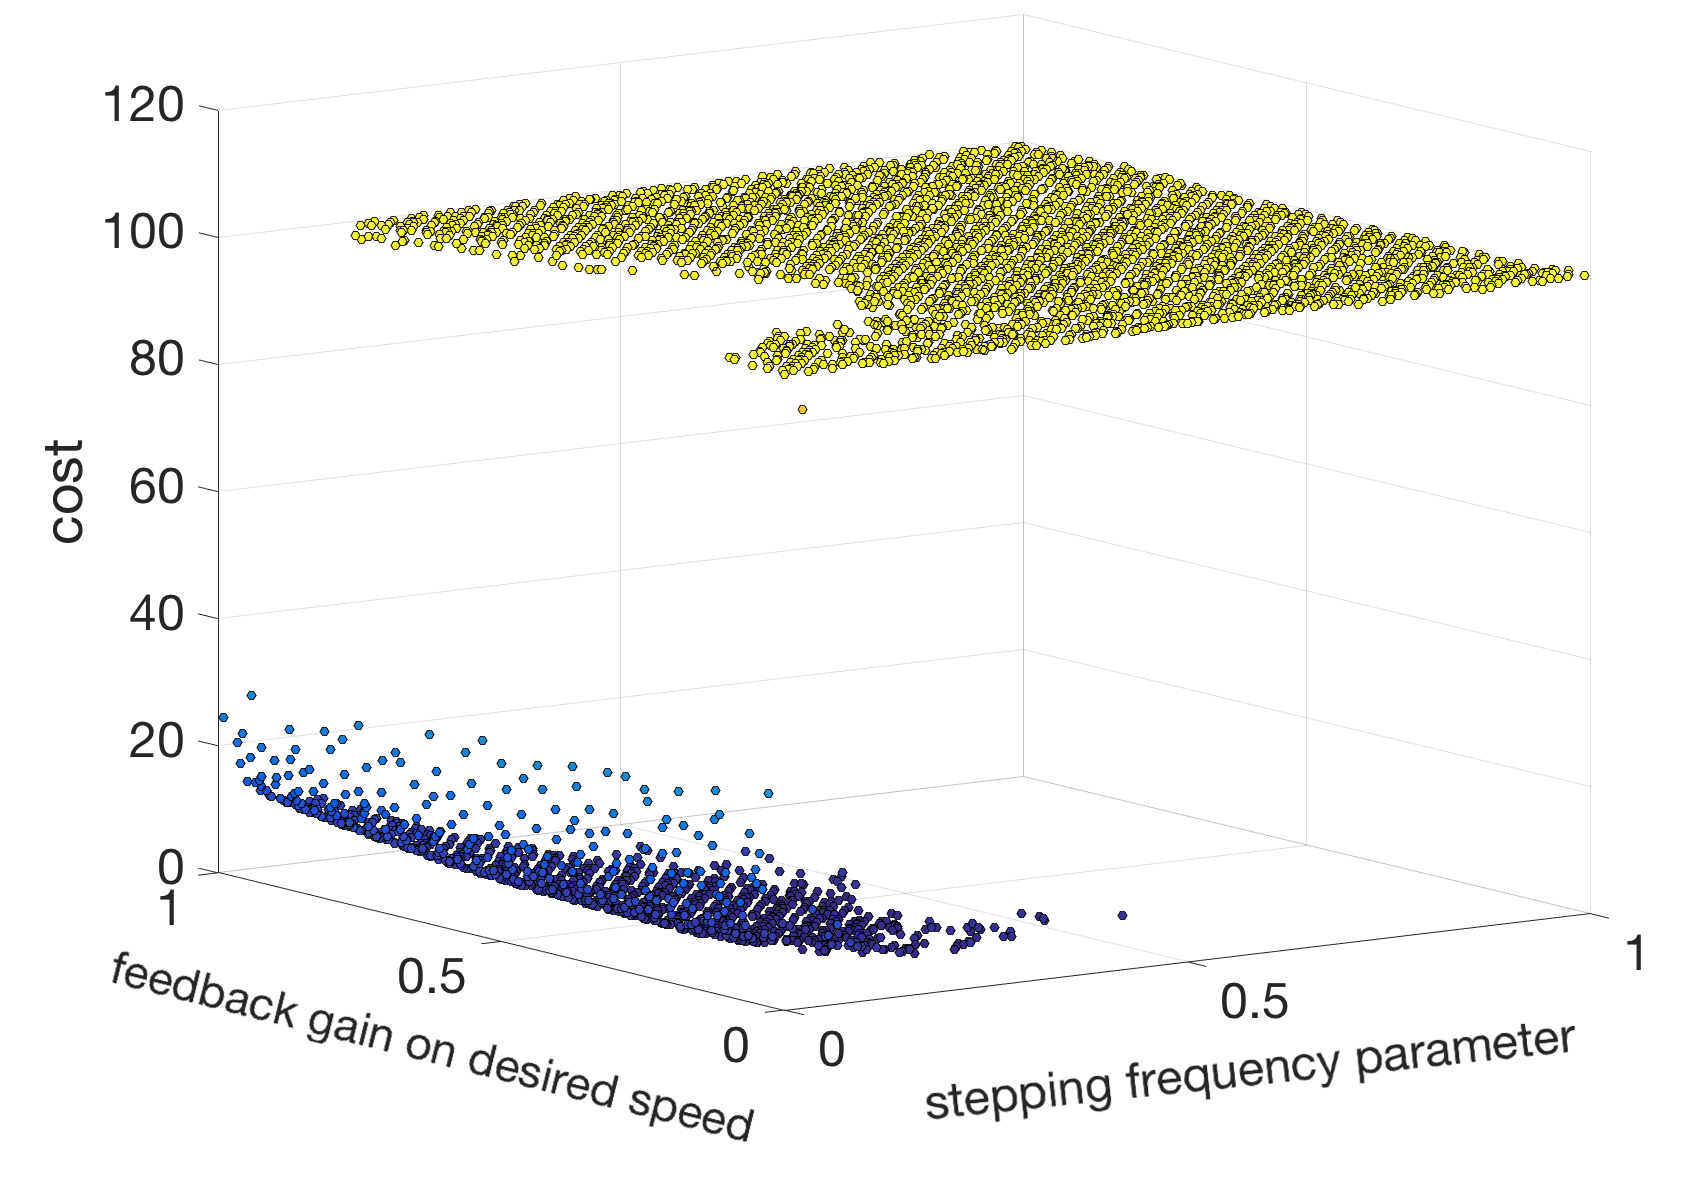
\includegraphics[width=0.7\textwidth]{img/costs_atrias.png}
\label{fig:atrias_cost_landscape}
\end{figure}

Figure~\ref{fig:atrias_cost_landscape} shows a scatter plot of applying cost from Equation~\ref{eq:cost_atrias} to simulations of a 5-dimensional controller for the ATRIAS robot as introduced in Section~\ref{sec:raibert_cont}. For visualization we only vary the 2 most sensitive dimensions, leading to a 2-dimensional subspace of the parameter space. We pick a successful controller (in 5D), then vary the first two dimensions - the stepping frequency of the controller and the feedback gain on the desired speed. As seen in the figure, less than a quarter of this subspace contains points corresponding to low-cost simulation results (blue points on the scatter plot). 

The challenge comes from the fact that the boundary between the well-performing (blue) and poorly performing (yellow) parameters is discontinuous. This is a typical landscape for bipedal systems, where a controller that makes the robot fall is much worse than one that walks, and the boundary is extremely sharp. While there can be variations to how costs are structured among stable walking points -- efficiency vs speed vs distance covered, parameters that fall are much worse than those who don't. Fitting such cost function with regression can be difficult. Learning to reconstruct the boundary exactly using the training set might result in overfitting and poor performance on the test set. Trying to fix this by applying regularization is likely to result in high loss and uncertainty about the points close to the boundary. This is particularly problematic if poorly performing points lie close to some of the most promising regions of the parameter space, which is the case for the setting we consider. 
%\begin{figure}[t]
%\centering
%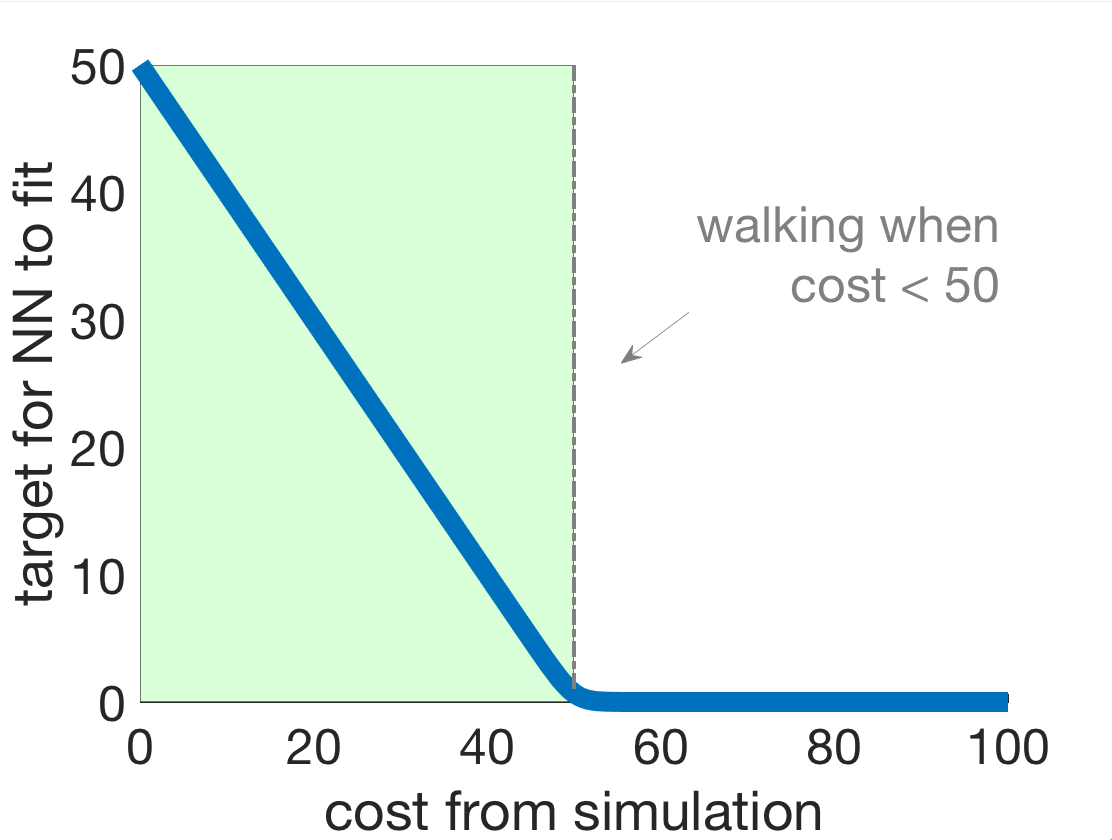
\includegraphics[width=0.35\textwidth]{img/softplus.png}
%\caption{\small{Softplus Cost transformation.}}
%\label{fig:atrias_cost_transform}
%\end{figure}
%Instead of a straightforward approach of learning to reconstruct the cost function directly, 
We propose to use a transformation of the cost as the target for the supervised learning. Our approach is to train a deep neural network to reconstruct a reflected shifted softplus function of the cost: 
\begin{equation}
\textit{score}_{\textit{NN}} = \zeta \big( cost_{walk} - cost_{sim}(\pmb{x}) \big)
\label{eq:score_asymnn}
\end{equation}
Here $\zeta$ is a softplus function: $\zeta(a) = ln\big( 1 + e^a \big)$, $cost_{walk}$ is the average cost for the parameter sets that walk during short simulations, $cost_{sim}(\pmb{x})$ is the cost computed by the simulator for vector $\pmb{x}$ of controller parameter values (Eq. \ref{eq:cost_atrias}). Using this transformation yields a ``score" function such that parameter sets which produce poor results in simulation are mapped to values close to zero. With this, the differences in scores of the poorly performing parameter sets become small or zero. In contrast, the differences in scores of the parameter sets yielding potentially promising results remain proportional to the difference in the corresponding costs. %Figure~\ref{fig:atrias_cost_transform} gives a visualization of this transformation.

Cost transformation in Equation~\ref{eq:score_asymnn} serves to essentially create an asymmetric loss for neural network training. This asymmetric loss is minimized when the promising (low-cost, high-score) points are reconstructed correctly.
%yielding linear relationship between the transformed scores and the original costs. 
For the poorly performing (high-cost, low-score) points, it only matters that the output of the neural network is close to zero. Such asymmetric loss can be interpreted as implementing a hybrid of regression and ``soft'' classification. The regression aspect aims to fit the promising points which correspond to parameters yielding walking behaviors. The ``soft'' classification causes an increase in the loss only if a poorly performing point is ``mis-classified'' as well-performing (output of the neural network is not close to zero). As a result, while the network still tries to perfectly fit the well performing points, it only needs to classify poorly performing points as poor.

The asymmetry in the loss is essential for training to reconstruct noisy costs with sharp discontinuities. Such cost functions are frequently used in optimization of locomotion controllers, with the aim to sharply penalize falling. This challenge is further addressed by learning to reconstruct the transformation of the cost (as discussed above) in combination with using a L1 loss, instead of the usual L2 loss when training the neural network. With this, errors in reconstructing points on the boundary contribute only linearly to the overall loss. This helps achieve a better fit of the stable parts of the parameter space, instead of focusing on the boundary.
%avoid focusing too much on fitting the hard-to-reconstruct uncertain region in favor of learning a better fit of other more stable parts of the parameter space.

The resultant transform $\phi(\pmb{x})$ from this cost based transform is the output of the neural network:
\begin{equation}
    \phi(\pmb{x}) = score_{NN}(\pmb{x})
\end{equation}


We utilize the reconstructed transformed costs to define $\textit{asymNN}$ kernel for Bayesian optimization:
\begin{align}
    k(\pmb{x}_i, \pmb{x}_j) \rightarrow k(\phi(\pmb{x}_i), \phi(\pmb{x}_j)) \\
    k_{asymNN}(\pmb{x}_i, \pmb{x}_j) = \sigma_k^2 \exp\Big(- \frac{1}{2 \pmb{l}^2} \|\phi(\pmb{x}_i) - \phi(\pmb{x}_j)\|^2 \Big),
\end{align}
with hyperparameters $\sigma_k, \pmb{l}$.
The proposed approach is able to clearly separate the unpromising part of the parameter space. Under the resulting distance metric poorly performing sets of parameters are close together and far from well-performing ones. 
A smaller priority is given to high-precision reconstruction of the poorly performing region of the parameter space. This is desirable, since it has been observed that usually simulators are optimistic compared to the real word~\citep{cutler2015real}. This is indeed the case with the locomotion simulators we consider: if a set of controller parameters causes falling or instability in simulation, it is very unlikely that the same controller parameters would result in successful walking when applied to real hardware. With that, distinguishing all the various ways in which poorly performing points fail is not useful. Using \textit{asymNN} kernel helps rapidly separate bad regions of the parameter space from the regions that might contain promising points. 

\subsubsection{Reconstructing Cost-agnostic Trajectory Summaries}
\label{sec:approach_traj}

While learning a distance metric from the cost could be effective for a wide variety of problems, frequently there is a need for a cost-agnostic approach. Such cases arise when the data from the simulator is computationally expensive to collect and we need to change the cost function. Different tasks might call for slightly different cost functions. For example, high energy consumption could be penalized if energy use needs to be restricted; robustness of the walk could be emphasized if only stable walking is acceptable; if achieving the desired speed is the most important factor -- then the cost might instead only reflect how well the desired speed is maintained. For such cases we propose to train a neural network to reconstruct summaries of trajectories that are cost-agnostic, then utilize these trajectory summaries for constructing kernel distance metrics.

In most cases, a summary of trajectory information contains all the pertinent information. Hence, we focus on collecting the following aspects of the simulated trajectories: walking time (time before falling), energy used during walking, position of the torso, angle of the torso, coordinates of the center of mass at the end of the short simulation runs. These summaries of simulated trajectories are collected for a range of controller parameters and comprise the training set for the neural network to fit (input: $\pmb{x}$ -- a set of control parameters; output: $\pmb{traj_x}$ -- the corresponding trajectory summary obtained from simulation). The outputs of the (trained) neural network offer the reconstructed/approximate trajectory summaries:
\begin{equation}
    score_{\textit{trajNN}}(\pmb{x}) = \pmb{\widehat{traj}_x}
\end{equation}
where $\pmb{x}$ is the input controller parameters, and $\pmb{\widehat{traj}_x}$ is the corresponding reconstructed trajectory summary.
These are then used to define a distance metric for the kernel for Bayesian Optimization:
\begin{align}
\phi(\pmb{x}) = score_{trajNN}(\pmb{x})\\
k_{\textit{trajNN}}(\pmb{x}_i, \pmb{x}_j) = \sigma_k^2 \exp\Big(- \frac{1}{2 \pmb{l}^2} \|\phi(\pmb{x}_i) - \phi(\pmb{x}_j)\|^2 \Big)
\end{align}
with hyperparameters $\sigma_k, \pmb{l}$ .

The general concept of utilizing trajectory data to improve sample efficiency of BO has been proposed before, for example in~\cite{wilson2014using}. However, prior work assumed obtaining trajectory data is possible every time kernel values $k(\pmb{x}_i, \pmb{x}_j)$ need to be evaluated. This is not the case in our setting, as each controller has to be evaluated to obtain the simulation trajectory. To overcome this, we obtain trajectory summaries via costly high-fidelity simulations. To avoid having to run simulations while performing BO on hardware, we train a neural network to learn reconstructing trajectory summaries first. Running a forward pass of the neural network is a relatively inexpensive operation, hence reconstructed/approximate trajectory summaries can be quickly obtained during BO whenever $k_{\textit{trajNN}}(\pmb{x}_i, \pmb{x}_j)$ needs to be computed. Note that the trajectory information we extract is generic and can be applied to other problems without requiring in-depth domain knowledge. When applying this approach to a new domain, the strategy would be to include trajectory information used to compute cost functions that are of interest/relevance in the domain. For example, for a manipulator, the coordinates of  end-effector(s) could be recorded at relevant points.

In addition to offering a cost-agnostic approach, our trajectory-based kernel retains more information about important aspects of simulated trajectories than a cost-based  kernel. We observe that this re-parameterization could be more effective than a cost-based kernel in cases when the kernel does not retain enough information to effectively optimize the acquisition function used in Bayesian Optimization, due to over-condensing the characteristics of the simulation. In particular, a cost-based kernel offers most sample-efficient results in the case of using lower-dimensional controller and the case of using a smooth cost with a higher-dimensional controller - basically easy to optimize problems. On more challenging discontinuous costs and high-dimensional controllers, trajectory-based kernels outperform cost-based kernels, as they do not condense the whole space of controllers to a single point. Thus, they are capable of recovering from some mismatch between simulation and hardware to some extent. 
The trajectory-based kernel also significantly outperforms standard Bayesian Optimization, even when the optimization uses challenging discontinuous costs. 
%In the experiments section we compare the performance of the kernel based on 8-dimensional trajectory summaries with that of a 1-dimensional cost-based kernel. 

%\AR{Add the pipeline picture at the top of this page.}

\section{Modelling mismatch between simulation and hardware}
\label{sec:mismatch}
While all the generalized transforms $\phi$ proposed in the previous section can successfully characterize the quality of a gait, large mismatch between a simulator and real-world hardware could still present a challenge. Some controller parameters could yield good gait characteristics in a short simulation, but perform poorly during a longer trial on hardware or simulation. While this issue did not arise during our hardware experiments with the controller described in Section~\ref{sec:raibert_cont}, this could be an issue with a different and higher-dimensional controller and inaccurate simulator. Hence, it is important to study how the performance worsens as the fidelity of the simulator decreases and how the kernel can be adjusted to compensate for this mismatch.

In ~\cite{rai2017bayesian}, we proposed a way to incorporate information about simulation-hardware mismatch into the kernel from the samples evaluated so far. We augment the simulation-based kernel to include this additional information about mismatch, by expanding the original kernel by an extra dimension that contains the predicted mismatch for each controller $\pmb{x}$.
 
A separate Gaussian process is used to model the mismatch experienced on hardware, starting from an initial prior mismatch of 0: $g(\pmb{x})\!\sim\!\mathcal{GP}(0, k_{SE}(\pmb{x}_i,\pmb{x}_j))$.
For any evaluated controller $\pmb{x}_i$, we can compute the difference between $\phi(\pmb{x}_i)$ in simulation and on hardware: 
\begin{equation}
    d_{\pmb{x}_i}\!=\!\phi^{sim}(\pmb{x}_i) \!-\! \phi^{hw}(\pmb{x}_i)    
\end{equation}
 
We can now use mismatch data $\{ d_{\pmb{x}_i} | i=1...n \}$ to construct a model for the expected mismatch: $\bar{g}(\pmb{x})$. In the case of using a GP-based model, $\bar{g}(\cdot)$ would denote the posterior estimate of expected mismatch. With this, we can predict simulation-hardware mismatch in the original space of controller parameters for unevaluated controllers. Combining this with kernel $k_{\phi}$ we obtain an adjusted kernel:
\begin{align}
\label{eq:k_adj}
    \pmb{\phi}^{adj}_{\pmb{x}} = \begin{bmatrix} \phi^{sim}(\pmb{x}) \\ \bar{g}(\pmb{x}) \end{bmatrix}, \quad \quad \quad \quad \quad \quad 
    \pmb{t}_{ij}^{adj} \!=\! \pmb{\phi}^{adj}_{\pmb{x}_i} \!-\! \pmb{\phi}^{adj}_{\pmb{x}_j} \\
    k_{\phi_{adj}}(\pmb{x}_i, \pmb{x}_j) = \sigma_k^2 \exp\Big(- \tfrac{1}{2} (\pmb{t}_{ij}^{adj})^T \diag\Big(\begin{bmatrix}\pmb{\ell_1} \\ \pmb{\ell_2} \end{bmatrix}\Big)^{\!-\!2} \pmb{t}_{ij}^{adj} \Big) \\
\end{align}

The similarity between points $\pmb{x}_i, \pmb{x}_j$ is now dictated by two components: representation in $\phi$ space and expected mismatch. This construction has an intuitive explanation: Suppose controller $\pmb{x_i}$ results in walking when simulated, but falls during hardware evaluation. $k_{\phi_{adj}}$ would register a high mismatch for $\pmb{x}_i$. Controllers would be deemed similar to $\pmb{x}_i$ only if they have both similar simulation-based $\phi(\cdot)$ and similar estimated mismatch $\bar{g}(\cdot)$. Points with similar simulation-based $\phi(\cdot)$ and low predicted mismatch would still be `far away' from the failed $\pmb{x}_i$. This would help BO sample points that still have high chances of walking in simulation, but are in a different region of the original parameter space that $\pmb{x}_i$. In the next section, we present a more mathematically rigorous interpretation for $k_{\phi_{adj}}$.




%With this construction, if there is a mismatch in simulation vs hardware, the problematic region will have a high adjusted DoG kernel distance to regions without the mismatch.
We will call this adjusted kernel with hardware and simulation mismatch the adjusted \dogkernel in the future.
This formulation is similar in spirit to other approaches, such as \cite{marco2017virtual}. However, while previous work ``mistrusts" all simulation data, our formulation lets us fit a dynamic mismatch function from data. This lets us trust the simulation in some regions, while mistrust it in others.

There are several approaches in literature that attempt to model the difference between simulation and hardware. \cite{wilson2014using} propose modelling the mismatch between a learned model and the real system by a second ``residual" GP. They predict the expected cost at a new point using a convex combination of two GPs:  
\begin{align}
    J(\pmb{x}) = (1-\beta) J_{sim}(\pmb{x}) + \beta J_{err}(\pmb{x}) \\
    J_{err}(\pmb{x}) \sim \mathcal{GP}(0, k(\pmb{x},\pmb{x}')) \\ 
    J_{sim}(\pmb{x}) \sim \mathcal{GP}(m_{sim}(\pmb{x},\pmb{x}_i,...,\pmb{x}_n), k(\pmb{x},\pmb{x}'))
\end{align}
$\beta$ can be learned from data. $J_{err}$ models the residual between the simulation model and the actual data, initialized with a 0 prior. $J_{sim}$ is a cost model learned over simulation points $m_{sim}(\pmb{x},\pmb{x}_i,...,\pmb{x}_n)$, which are be an inaccurate representation of the actual system. The resultant GP has a mean which is a convex combination of the two GP means, and the same variance as the chosen $k$. While this approach can be very powerful when the simulation is close to hardware, with significant mismatch the bias of simulation can be hard to overcome.

In contrast, our approach puts majority of the information from simulation into the kernel, which is an easier to overcome biased prior information. We present a more mathematical foundation for our mismatch model in the next section. Results comparing our approach to other approaches from literature are in Section \ref{subsec:sim_experiments_prior_cully}


Multiple sources of information can also be added to Gaussian Processes \citep{poloczek2016multi}. For example, let the true cost be a combination of cost in simulation and a residual error - each with a separate kernel:
\begin{equation}
    J(\pmb{x}) = J_{sim}(\pmb{x}) + J_{err}(\pmb{x})
\end{equation}
where
\begin{align}
     J_{err}(\pmb{x}) &\sim \mathcal{GP}(0, k_{err}(\pmb{x},\pmb{x}')) \\
J_{sim}(\pmb{x}) &\sim \mathcal{GP}(\mu_{sim}(\pmb{x}), k_{sim}(\pmb{x},\pmb{x}'))
\end{align}

Here $J(\pmb{x})$ is the true cost of the controller on hardware, $J_{sim}(\pmb{x})$ is a measurement from simulation, and $J_{err}(\pmb{x})$ is the noise distribution, which is the mismatch between simulation and hardware. Points sampled from hardware do not have this mismatch, and hence are samples from the true GP $J(\pmb{x})$. However points from simulation are samples from $J_{sim}(\pmb{x})$ and their corresponding residual $J_{err}$ needs to be estimated. 

\cite{poloczek2016multi} extend the kernel by an additional binary
variable $\delta$, which indicates whether the cost is evaluated in
simulation $(\delta = 0)$ or on the physical system $(\delta = 1)$. Based on the extended parameter $a = (\pmb{x}, \delta)$, we can model the cost
by adapting the kernel of $J$ to
\begin{equation}
    k(\pmb{x}, \pmb{x'}) = k_{sim}(\pmb{x}, \pmb{x'}) + \delta \delta' k_{err}(\pmb{x}, \pmb{x'})
\end{equation}
\cite{marco2017virtual} develop an automatic way of trading off data from simulation and hardware based on the expected improvement of each source, normalized by the time cost of sampling simulation vs hardware. 

For high dimensional controllers, these error maps can  need a lot of data to accurately model the inaccuracy of simulation, especially for rapidly changing discontinuous costs. To overcome this problem, it is worth exploring if characteristics of simulation can be used to create a prior mismatch. For example, controllers with higher impacts might have a high chance of falling on hardware even if they walk in simulation. Similarly, controllers that venture close to joint limits might be likely to fail on hardware, even if successful in simulation. 

In comparison, building a mismatch map for the reduced dimensional DoG-space can be very data efficient. This allows us to compensate for the mismatch between simulation and hardware and propogate this information back to update the features collected in simulation. This leads to a novel way of updating models from hardware data in a transformed space with very few data points. Moreover, if the simulation is close to hardware in some regions, the learned mismatch is close to 0 and higher in other regions where the simulation is different from the hardware.

\subsection{Interpretation of Kernel with Mismatch Modeling}

In this section we give a more mathematically sound interpretation the mismatch adjusted kernel described in the previous section.

Let us consider a controller $\pmb{x}_i$ evaluated on hardware. The difference between simulation-based and hardware-based feature transform for $\pmb{x}_i$ is $d_{\pmb{x}_i} = \phi^{sim}(\pmb{x}_i) - \phi^{hw}(\pmb{x}_i)$. The `true' hardware feature transform for $\pmb{x_i}$ is $\phi^{hw}(\pmb{x_i}) = \phi^{sim}(\pmb{x_i}) - d_{\pmb{x_i}}$. After $n$ evaluations on hardware, $\{ d_{\pmb{x}_i} | i=1...n \}$ can serve as data for modeling simulation-hardware mismatch. In principle, any data-efficient model $g(\cdot)$ can be used, such as GP (a multi-output GP in case $\phi(\cdot)$ $>1D$). With this, we can obtain an adjusted transform: $\hat{\phi}^{hw}(\pmb{x}) = \phi^{sim}(\pmb{x}) - \bar{g}(\pmb{x})$, where $\bar{g}(\cdot)$ is the output of the model fitted using $\{d_{\pmb{x}_i} | i=1,...n \}$.

Suppose $\pmb{x}_{new}$ has not been evaluated on hardware. We can use $\hat{\phi}^{hw}(\pmb{x}_{new}) = \phi^{sim}(\pmb{x}_{new}) - \bar{g}(\pmb{x}_{new})$ as the adjusted estimate of what the output of $\phi$ should be, taking into account what we have learned so far about simulation-hardware mismatch.

Let's construct kernel $k^{v_2}_{\phi_{adj}}(\pmb{x}_i, \pmb{x}_j)$ that uses these hardware-adjusted estimates directly:
\begin{equation*}
\begin{split}
\pmb{q}_{ij}^{adj} &= \hat{\phi}^{hw}(\pmb{x}_{i}) - \hat{\phi}^{hw}(\pmb{x}_{j}) \\
&= (\phi^{sim}(\pmb{x}_{i}) - \bar{g}(\pmb{x}_i)) - (\phi^{sim}(\pmb{x}_{j}) - \bar{g}(\pmb{x}_j) ) \\
&= \underbrace{(\phi^{sim}(\pmb{x}_{i}) - \phi^{sim}(\pmb{x}_{j}))}_{\pmb{v}_{\phi}} + \underbrace{(\bar{g}(\pmb{x}_j) - \bar{g}(\pmb{x}_i) )}_{\pmb{v}_{g}}
\end{split}
\end{equation*}

\begin{equation*}
\begin{split}
k^{v_2}_{\phi_{adj}}(\pmb{x}_i, \pmb{x}_j) &= \sigma^2_{k_{v_0}} \exp\Big(- \tfrac{1}{2} (\pmb{q}_{ij}^{adj})^T \diag(\pmb{\ell})^{\!-\!2} \pmb{q}_{ij}^{adj} \Big) \\
& = \sigma^2 \exp\Big(- \tfrac{1}{2} \big[ (\pmb{v}_{\phi} + \pmb{v}_{g})^T \diag(\pmb{\ell})^{\!-\!2} (\pmb{v}_{\phi} + \pmb{v}_{g}) \big] \Big) \\
& = \sigma^2
\exp\Big(- \tfrac{1}{2} \big[ \pmb{v}_{\phi}^T \diag(\pmb{\ell})^{\!-\!2} \pmb{v}_{\phi} + \pmb{v}_{g}^T\diag(\pmb{\ell})^{\!-\!2} \pmb{v}_{g} + prod_{ij} \big] \Big)\\
&\quad \quad \quad \quad \quad \text{where } prod_{ij} = 2 \pmb{v}_{\phi}^T\diag(\pmb{\ell})^{\!-\!2} \pmb{v}_{g}
\end{split}
\end{equation*}

Using $\exp(a+b+c)=\exp(c) \cdot \exp(a+b)$,  we have:
\begin{align*}
k^{v_2}_{\phi_{adj}}(\pmb{x}_i, \pmb{x}_j) &= \sigma^2 \exp(-prod_{ij}) \exp\Big(- \tfrac{1}{2} \big[ \pmb{v}_{\phi}^T \diag(\pmb{\ell})^{\!-\!2} \pmb{v}_{\phi} + \pmb{v}_{g}^T\diag(\pmb{\ell})^{\!-\!2} \pmb{v}_{g} \big] \Big)
\end{align*}

If we now observe that $\pmb{v}_{g}^T\diag(\pmb{\ell})^{\!-\!2} \pmb{v}_{g} = (-\pmb{v}_{g})^T\diag(\pmb{\ell})^{\!-\!2} (-\pmb{v}_{g})$ we get:
\begin{align*}
k^{v_2}_{\phi_{adj}}(\pmb{x}_i, \pmb{x}_j) 
&= \sigma^2 \exp(-prod_{ij}) \exp\Big(- \tfrac{1}{2} (\pmb{t}_{ij}^{adj})^T \diag\Big(\begin{bmatrix}\pmb{\ell} \\ \pmb{\ell} \end{bmatrix} \Big)^{\!-\!2} \pmb{t}_{ij}^{adj} \Big) \\
\pmb{t}_{ij}^{adj} &= 
\begin{bmatrix}
\phi^{sim}(\pmb{x}_{i}) - \phi^{sim}(\pmb{x}_{j}) \\
\bar{g}(\pmb{x}_i) - \bar{g}(\pmb{x}_j)
\end{bmatrix} \text{ (from Equation~\ref{eq:k_adj})}
\end{align*}

Compare this to $k_{\phi_{adj}}$ from Equation~\ref{eq:k_adj}:
\begin{equation}
k_{\phi_{adj}}(\pmb{x}_i, \pmb{x}_j) = \sigma_k^2 \exp\Big(- \tfrac{1}{2} (\pmb{t}_{ij}^{adj})^T \diag\Big(\begin{bmatrix}\pmb{\ell_1} \\ \pmb{\ell_2} \end{bmatrix}\Big)^{\!-\!2} \pmb{t}_{ij}^{adj} \Big)
\end{equation}
Now we see that $k^{v_2}_{\phi_{adj}}$ and $k_{\phi_{adj}}$ have a similar form. Hyperparameters $\pmb{\ell_1}, \pmb{\ell_2}$ provide flexibility in $k_{\phi_{adj}}$ as compared to having only vector $\pmb{\ell}$ in $k^{v_2}_{\phi_{adj}}$. They can be adjusted manually or with Automatic Relevance Determination \citep{GPsMLBook}. 
For $k^{v_2}_{\phi_{adj}}$, the role of signal variance is captured by $\sigma^2 \exp(-prod_{ij})$. This makes the kernel nonstationary in the transformed $\phi$ space. 
Since $k_{\phi_{adj}}$ is already non-stationary in $\pmb{x}$, it is  unclear whether non-stationarity of $k^{v_2}_{\phi_{adj}}$ in the transformed $\phi$ space has any advantages.

The above discussion shows that $k_{\phi_{adj}}$ proposed in ~\cite{rai2017bayesian} is motivated both intuitively and mathematically. It aims to use a transform that accounts for the hardware mismatch, without adding extra non-stationarity in the transformed space. It also helps propagate data seen on hardware back to simulation, thus updating simulation models in a sample-efficient manner. If one has intuitions about the mismatch in the space of controllers, they could be used in the prior of the mismatch kernel to improve sample-efficiency further. 

\section{Transfer learning with contextual Bayesian optimization}


It is possible to transfer knowledge between tasks using Bayesian optimization by adding context to the learning. Contexts can include specific features of the experiment such as target speed of walking, or the incline of the ground. In such cases, the cost observed on hardware is a function of not just the controller parameters $\pmb{x}$, but also the context $c$, leading to a cost of the form $f(\pmb{x},c)$. Since the context is an observed variable, and not an optimized variable, Bayesian optimization is done on the parameters $\pmb{x}$, which conditioning the posterior of the GP on the observed $c$.

\begin{align}
    f(\pmb{x},c) \sim \mathcal{GP}(\mu(\pmb{x}, c), k((\pmb{x},c),(\pmb{x}',c'))) \\
    \pmb{x}_{t+1} = \argmax EI(f(x,c)|c=c_{observed})
\end{align}

Additionally, the feature transform in simulation can be a function of $c$, as well as the updates learned on hardware. The features observed on hardware $\phi^{w}(\pmb{x}, c)$ depend on both the controller as well as context. Hence the mismatch GP is also a function of both as $d_{\pmb{x}_i, c} = \phi^{sim}(\pmb{x_i},c)- \phi^{hw}(\pmb{x_i},c)$. Even if we do not know the contexts when calculating simulation features, the mismatch update gives us a way of building a context-dependant feature transform from data. Figure \ref{fig:context} shows an example where BO was conducted on 6 different target speeds for a 50-dimensional neuromuscular controller on the ATRIAS biped described in Section \ref{sec:VNMC_cont}.  


The target speeds were $[0.5, 1.0, 1.5, 0.75, 1.25, 0.25, 1.75] m/s$. Initial speeds of $[0.5, 1.0, 1.5]m/s$ were simulated for 10 trials while latter speeds were simulated for 5. 
As shown in the figure, fewer trials are needed to reliably reach walking controllers as more data is added to the GP. This shows that learning on other target speeds indeed speeds up the learning for future targets, even when extrapolating. Target speeds of  $[0.75, 1.25, 0.25, 1.75] m/s$ reach a mean cost of $11.96$ after 5 trials, as compared to a mean cost of $19.61$ for the initial target speeds.

\begin{figure}
    \centering
    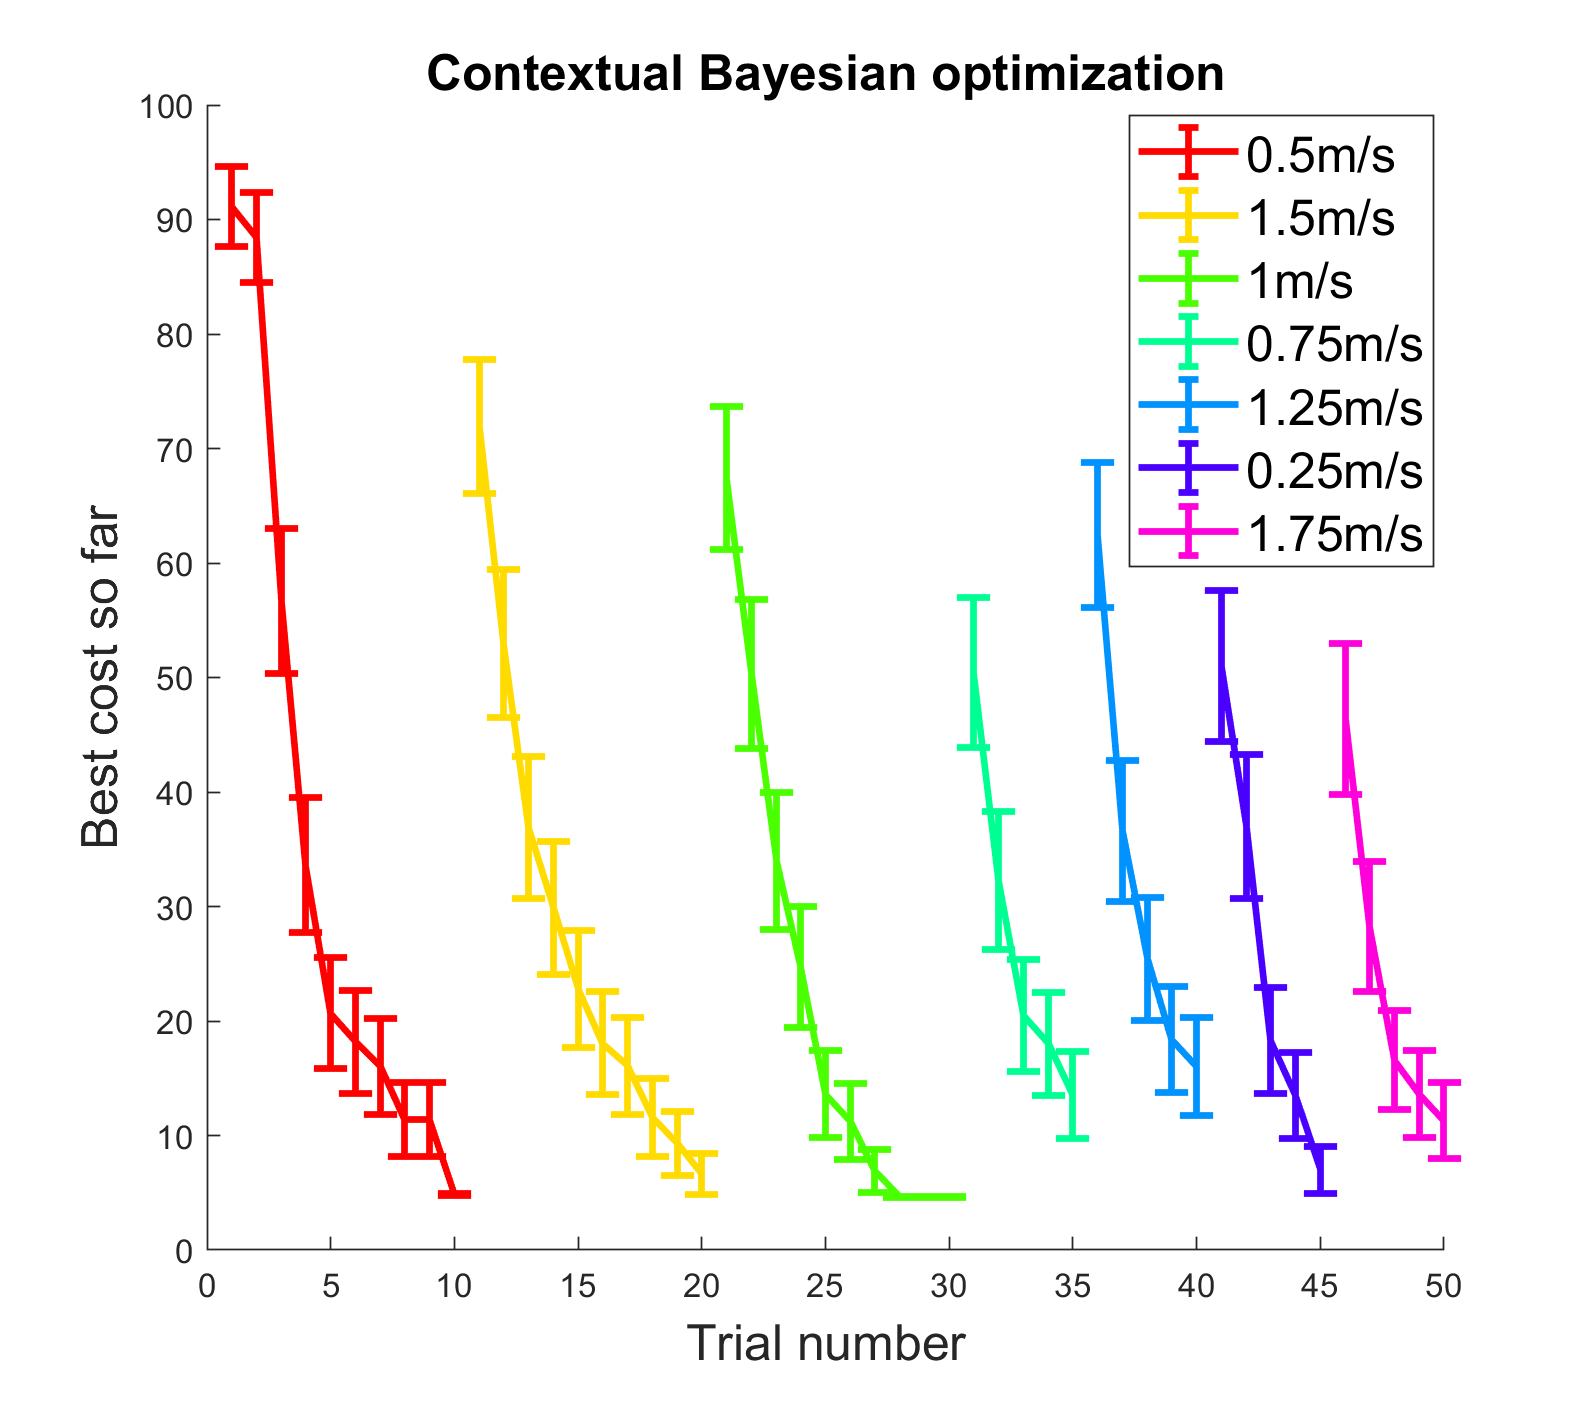
\includegraphics[width = 0.8\textwidth]{img/contexxt_bo.png}}
    \caption{Transfer learning with contextuan bayesian optimization can be used to transfer knowledge between different target speeds. Initial speeds of $[0.5, 1.0, 1.5]m/s$ were simulated for 10 trials while latter speeds of $[0.75, 1.25, 0.25, 1.75] m/s$ were simulated for 5 trials. The latter speeds reach a mean cost of $11.96$ after 5 trials, as compared to a mean cost of $19.61$ for the initial target speeds.}
    \label{fig:context}
\end{figure}